\documentclass[12pt,a4]{article}




\usepackage{graphicx,amsmath,amssymb,amsthm, boxedminipage,xcolor,amscd,amsbsy,latexsym,url,bm}

%\usepackage[lined,boxed]{algorithm2e}

\usepackage{algorithm}
\usepackage{algpseudocode}


\newtheorem{theorem}{Theorem}[section]
\newtheorem{proposition}[theorem]{Proposition}
\newtheorem{lemma}[theorem]{Lemma}
\newtheorem{corollary}[theorem]{Corollary}
\newtheorem{definition}[theorem]{Definition}

\newtheorem*{theorem*}{Theorem}
\newtheorem*{lemma*}{Lemma}
\newtheorem*{solution}{Solution}
\newtheorem*{proposition*}{Proposition}


\newtheorem{exercise}[theorem]{Exercise}
\newtheorem{exerciseD}[theorem]{*Exercise}
\newtheorem{exerciseDD}[theorem]{**Exercise}

\let\oldexercise\exercise
\renewcommand{\exercise}{\oldexercise\normalfont}

\let\oldexerciseD\exerciseD
\renewcommand{\exerciseD}{\oldexerciseD\normalfont}

%\let\oldexerciseD\exerciseD
%\renewcommand{\exerciseD}{\oldexerciseD\normalfont}

%\let\oldexerciseDD\exerciseDD
%\renewcommand{\exerciseDD}{\oldexerciseDD\normalfont}

\newcommand{\E}{\mathbb{E}}
%\newcommand{\nth}[1]{#1^{\textsuperscript{th}}}
\newcommand{\scalar}[2]{\ensuremath{\langle #1, #2\rangle}}
\newcommand{\floor}[1]{\left\lfloor #1 \right\rfloor}
\newcommand{\ceil}[1]{\left\lceil #1 \right\rceil}
\newcommand{\norm}[1]{\|#1\|}
\newcommand{\pfrac}[2]{\left(\frac{#1}{#2}\right)}
\newcommand{\nth}[1]{#1^{\textsuperscript{th}}}
\newcommand{\core}{\textnormal{core}}



\newif\ifsolution

\solutionfalse

\newcommand{\answer}[1]{
\ifsolution
{\color{blue} #1}
\else
\fi
}



\newcommand{\poly}{\textnormal{poly}}
\newcommand{\quasipol}{\textnormal{quasipol}}
\newcommand{\ssubexp}{\textnormal{stronglySubExp}}
\newcommand{\wsubexp}{\textnormal{weaklySubExp}}
\newcommand{\simplyexp}{\textnormal{E}}
\newcommand{\expo}{\textnormal{Exp}}



\newcommand{\N}{\mathbb{N}}
\newcommand{\nn}{\mathbb{N}_0^n}
\newcommand{\R}{\mathbb{R}}
\newcommand{\Z}{\mathbb{Z}}


\definecolor{darkgreen}{rgb}{0,0.6,0}

\date{}

\title{
\hbox{  Mathematical Foundations of Computer Science}
  \vspace{3mm}
{\normalsize CS 499,	Shanghai Jiaotong University,  Dominik Scheder\\
%\vspace{3mm}
Spring 2019}
}


\begin{document}

\maketitle

%\begin{quotation}
%  You are welcome to discuss the exercises in the discussion
%  forum. Please take them serious. Doing the exercises is as important
%  than watching the videos.
%
%  I intentionally included very challenging exercises and marked them
%  with one or two ``$*$''. No star means you should be able to solve
%  the exercises without big problems once you have understood
%  the material from the video lecture. One star means it requires 
%  significant additional thinking. Two stars means it is not 
%  unlikely that you will fail to solve them, even once you have understood
%  the material and thought a lot about the exercise. Don't feel bad
%  if you fail. Failure is part of learning.
%
%  This is the first time this course is online. Thus there might be mistakes
%  (typos or more serious conceptual mistakes) in the exercises. I will be 
%  grateful if you point them out to me!
%\end{quotation}


\newtheorem*{solution}{Solution}


\setcounter{section}{6}
\begin{center}
  \large\textbf{Group: navigator} 
\end{center}
\begin{center}
  \begin{tabular}{rl}
 Xu Huan  & 517021910724 \\
 Tianyao Shi     &     517021910623 \\
Chenxiao Yang    &    517021910540  \\
Jiaqi  Zeng      &     517021910882  \\
  \end{tabular}
\end{center}
\newpage
\section{Spanning Trees}





\subsection{Minimum Spanning Trees}


Throughout this assignment, let $G = (V,E)$ be a connected graph
and $w: E \rightarrow \R^+$ be a weight function.\\

\begin{exercise}
    Prove the inverse of the cut lemma: 
      If $X$ is good, $e \not \in X$, and $X \cup e$ is good,
      then there is a cut $S, V\setminus S$ such that (i) no
      edge from $X$ crosses this cut and (ii) $e$ is a minimum
      weight edge of $G$ crossing this cut.
\end{exercise}
\begin{proof}
	Since $X$ is good, $e \not \in X$, and $X \cup e$ is good(acyclic and totoal weight is smallest for $|X|+1$ edges, we guess?), we have $|X|<n-1$. Since we need at least $n-1$ edges to connect all vertices in a graph, there must exist a cut where no edge from $X$ crosses this cut, or we would use less than $n-1$ edges to connect all vertices, which is impossible. (i) is now proved. Then it is assumed that $e$ crosses such a not-crossed-by-any-edge-in-$X$ cut.
	
	For (ii), suppose $e$ is not a minimum weight edge of $G$ crossing this cut, say there exists some $e^{'}$ crossing this cut with $w(e)>w(e^{'})$. Then we cen infer that $X \cup e$ is not good since $X \cup e^{'}$ has smaller total weight. By contradiction, (ii) is correct.
\end{proof}
\begin{definition}
  For $c \in \R$ and a weighted graph $G = (V,E)$, let
  $G_c := (V, \{e \in E \ | \ w(e) \leq c\})$. That is, $G_c$ is the
  subgraph of $G$ consisting of all edges of weight at most $c$.
\end{definition}

\begin{lemma}
  Let $T$ be a minimum spanning tree of $G$, and let $c \in \R$.  Then
  $T_c$ and $G_c$ have exactly the same connected components.  (That
  is, two vertices $u,v \in V$ are connected in $T_c$ if and only if
  they are connected in $G_c$).
  \label{lemma-CC}
\end{lemma}

\begin{exercise}
     Illustrate Lemma~\ref{lemma-CC} with an example!
\end{exercise}

\textbf{Solution} \indent See Figure~\ref{fig:7.4}. In $G_3$, no edge crosses the cut, and so are E,F not connected in $T_3$. It's easy to see the lemma holds for $c$ equals other cases.
\begin{figure}[hbp]
	\centering
	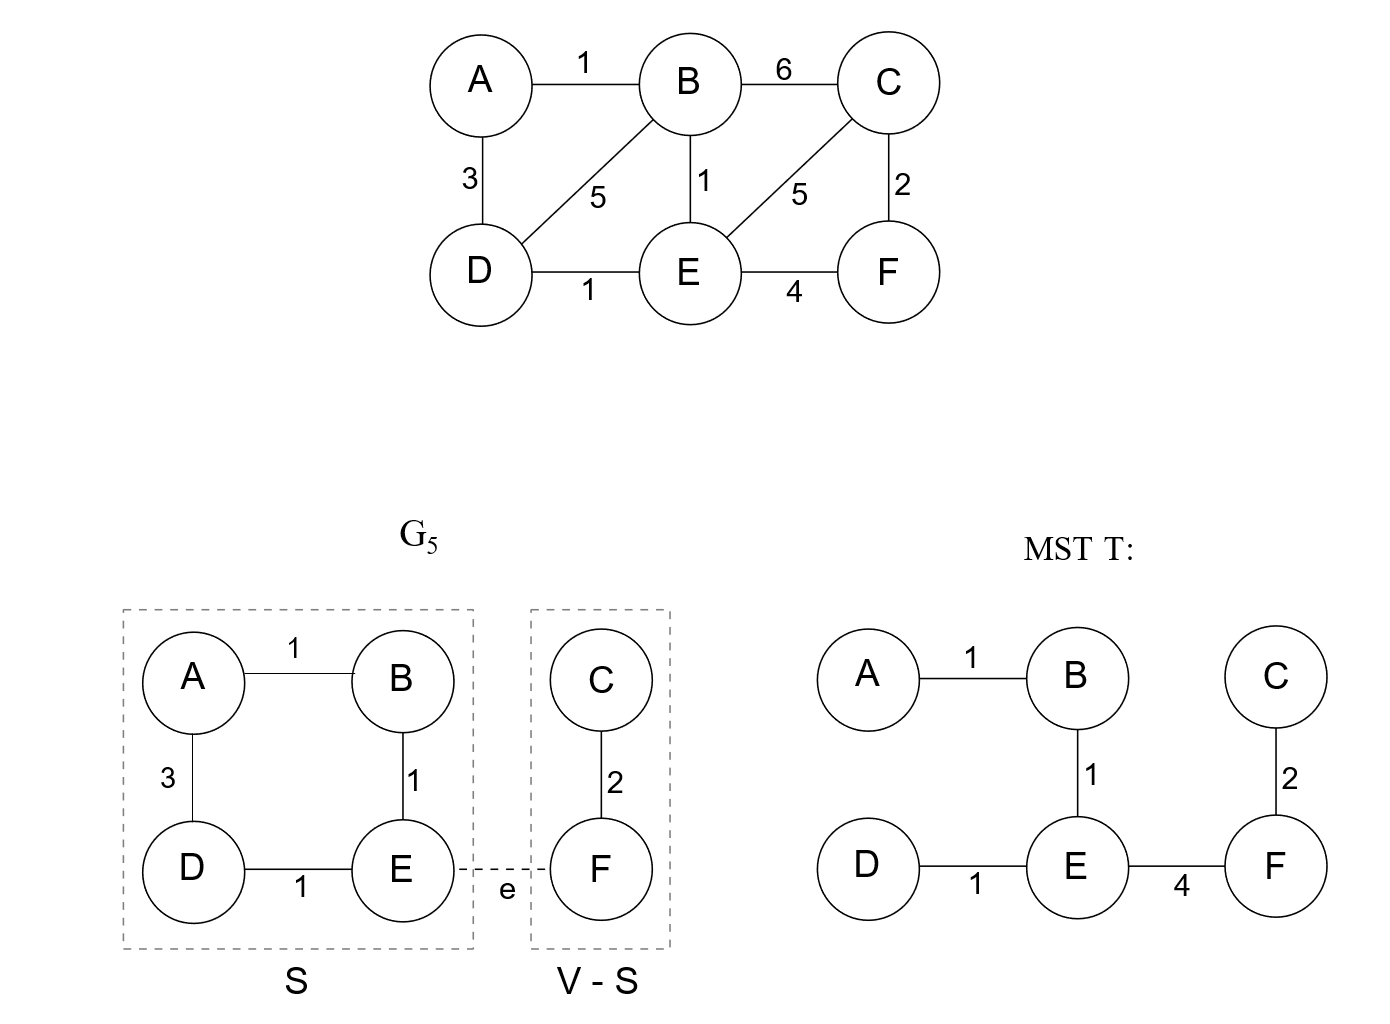
\includegraphics[width=0.8\textwidth]{figures/7_3.PNG}\label{fig:7.4}
	\caption{An illustration for Lemma 7.3. Figure source: \text{https://en.wikipedia.org/wiki/Minimum\_spanning\_tree} }
\end{figure}
\begin{exercise}
     Prove the lemma.
\end{exercise}
\begin{proof}
	\textbf{Necessity} If two vertices are connected in $T_c$, then the edges on the path between the two vertices $\in E$, all satisfying $w(e)\leq c$, which indicates they are also in $G_c$. Therefore in $G_c$ the two vertices are also connected.
	
	\textbf{Sufficiency} Suppose that two vertices are connected in $G_c$ yet not in $T_c$. This suggests that there exists some edge $e$ with $w(e)\leq c$ connecting the two vertices in $G$, and in the original $T$ weights of edges on the path between the two vertices is greater than $c$. If we replace the path in $T$ with that in $G_c$, we get a smaller minimum spanning tree, which is contradictory.    
\end{proof}
\begin{definition}
  For a weighted graph $G$, let $m_c(G) := | \{ e \in E(G) \ | \ w(e) \leq c\}|$, i.e.,
  the number of edges of weight at most $c$ (so $G_c$ has $m_c(G)$ edges).
\end{definition}

\begin{lemma}
  Let $T, T'$ be two minimum spanning trees of $G$. Then
  $m_c(T) = m_c(T')$.
  \label{lemma-weight-multiplicity}
\end{lemma}

\begin{exercise}
Illustrate Lemma~\ref{lemma-weight-multiplicity} with an example!
\end{exercise}

\textbf{Solution} \indent See Figure~\ref{fig:7.6}.Let the left MST be $T$ and another $T'$, $m_1(T) = m_1(T')=1$, $m_2(T) = m_2(T')=m_3(T) = m_3(T')=2$, $m_4(T) = m_4(T')=4$, $m_5(T) = m_5(T')=5$.
\begin{figure}[hbp]
	\centering
	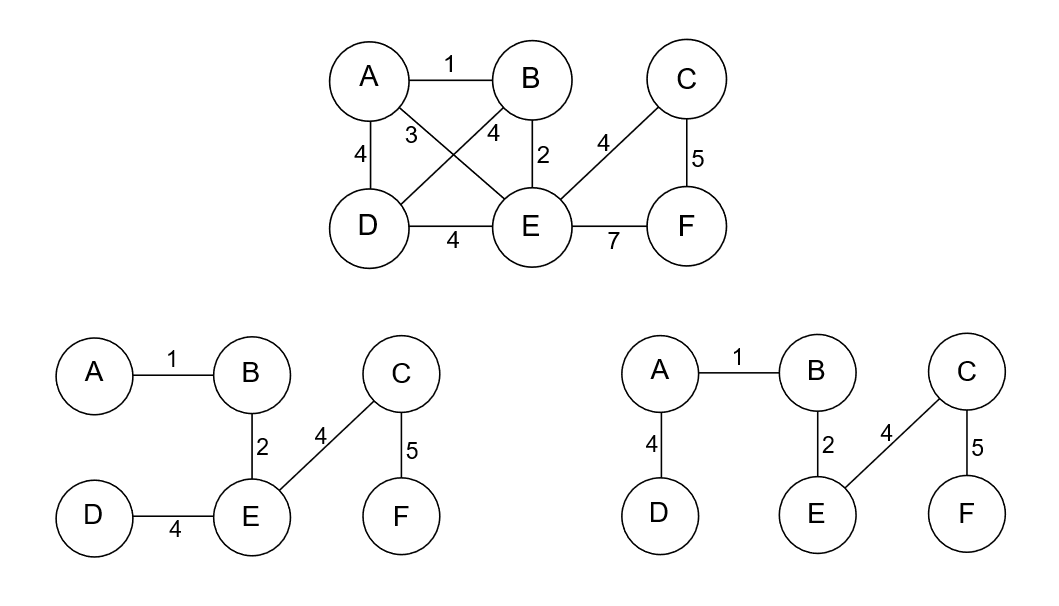
\includegraphics[width=0.8\textwidth]{figures/7_6.PNG}\label{fig:7.6}
	\caption{An illustration for Lemma 7.7. Figure source: https://en.wikipedia.org/wiki/Minimum$\_$spanning\_tree}
\end{figure}
\begin{exercise}
Prove the lemma.
\end{exercise}
\begin{proof}
	Assume that for two minimum spanning tree $T$, $T'$, $\exists c$ s.t. $m_c(T)\neq m_c(T')$. Without loss of generality, say $m_c(T)< m_c(T')$, and $c_0$ is the first $c\in \N$ s.t. $m_c(T)< m_c(T')$. Say it is edge $a$ with $w(a)=c_0$, so that $a\notin T$ yet $a\in T'$. Add $a$ to $T$ we must get a cycle, otherwise $a$ would belong to $T$, as all other edges would have weight greater than $a$. Grab this cycle we can see there is at least one edge $a'$ that is in $T$ yet not in $T'$. And $a'$ must have weight smaller than $a$, since $a$, corresponding to $c_0$, is the first to appear resulting in $m_c(T)< m_c(T')$. Replacing $a$ with $a'$ in $T'$ will result in a smaller minimum spanning tree, which is contradictory.
\end{proof}

\begin{exercise}
  Suppose no two edges of $G$ have the same weight. 
  Show that $G$ has exactly one minimum spanning tree!
\end{exercise}
\begin{proof}
	Assume that $G$ has more than one unique minimum spanning tree, $T,T'$. They have the same nodes yet different edges, since they are diffrent. Therefore there are at least two edges that belongs to one tree but not another. Let $e$ be the one with the smallest weight in such edges, and without loss of generality, say that $e \in T$. Add $e$ to $T'$ we get a cycle $C$ containing $e$, which also contains at least one edge $e'$ that is not in $T$. Since $e$ is chosen as the unique one with smallest weight, replace $e'$ with $e$ breaks the cycle to regain a minimum spanning tree, but with total weights smaller than $T'$, which is contradictory.
\end{proof}



\subsection{Counting Special Functions}

In the video lecture, we have seen a connection between functions $f: V \rightarrow V$
and trees on $V$. We used this to learn something about the number of such trees.
Here, we will go in the reverse direction: the connection will actually teach us a bit
about the number of functions with a special structure.\\

Let $V$ be a set of size $n$. We have learned that there are $n^n$ functions $f: V \rightarrow V$.
For such a function we can draw an ``arrow diagram" by simply drawing an arrow from
$x$ to $f(x)$ for every $V$. For example, let $V = \{0,\dots,7\}$ and $f(x) := x^2 \mod 8$.
The arrow diagram of $f$ looks as follows:
\begin{center}
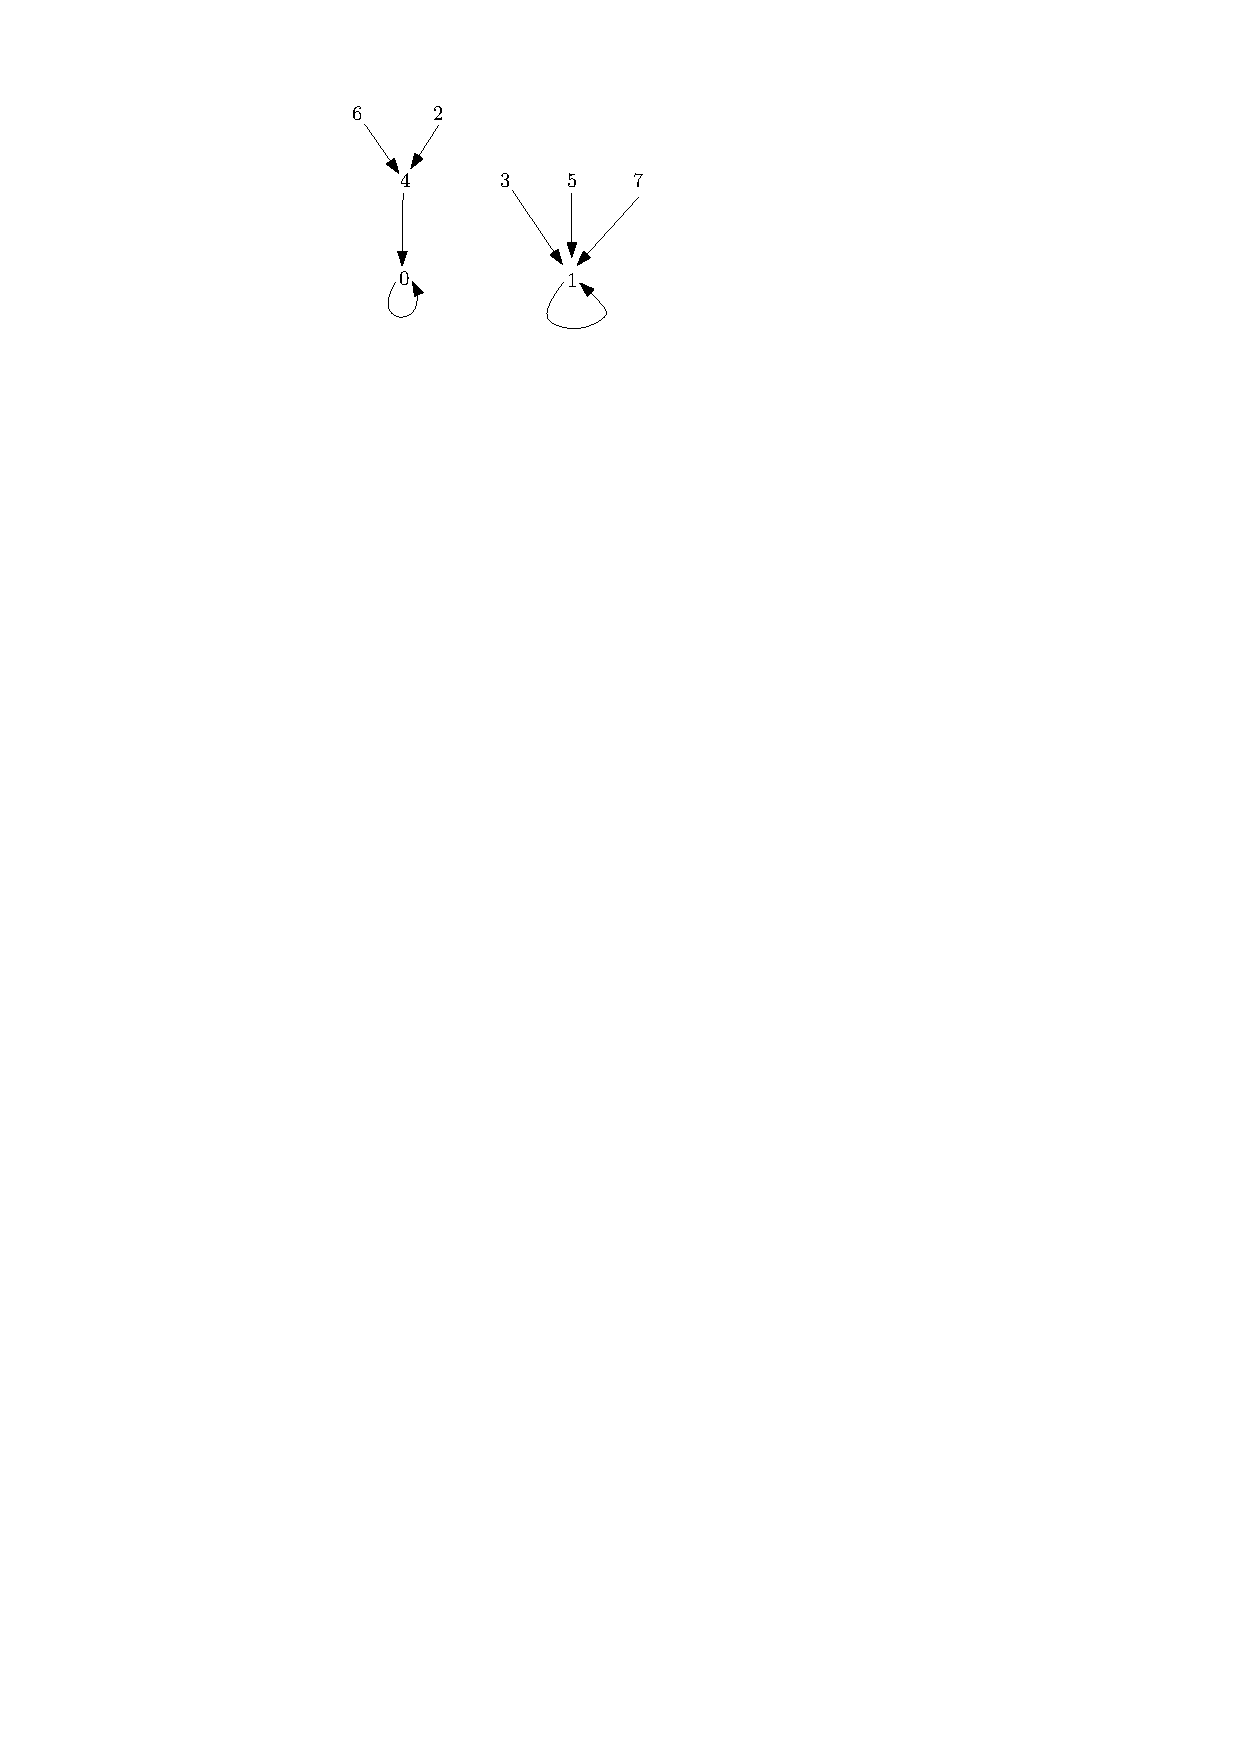
\includegraphics[width=0.3\textwidth]{figures/arrow-diagram.pdf}
\end{center}
The {\em core} of a function is the set of elements lying on cycles in such a diagram.
For example, the core of the above function is $\{0,1\}$. Formally, the core of $f$ is the 
set
\begin{align*}
%\core(f) = 
\{x \in V \ | \ \exists k \geq 1 f^{(k)}(x) = x \}
\end{align*}
where $f^{(k)}(x) = f( f( \dots f(x) \dots ))$, i.e., the function $f$ applied $k$ times 
iteratively to $x$.

\begin{exercise}
Of the $n^n$ functions from $V$ to $V$, how many have a core of size $1$? 
Give an explicit formula in terms of $n$.
\end{exercise}


\textbf{Solution.}
Recall that in the video lecture, we construct a function $f:V\rightarrow V$ according to the spanning tree and its vertebrate. For each spanning tree, there are totally  $n^2$ corresponding vertebrates. Among those vertebrates, there are $n$ vertebrates whose head and butt is the same vertex. In this case, the core-size of the corresponding function is $1$.\par 
As we know, there are totally $n^{n-2}$ spanning tree. For each spanning tree, there are $n$ required functions. Therefore, the total function number is $n^{n-2} \times n=n^{n-1}$.
%--------------------------- END ---------------------------

\begin{exercise}
How many have a core of size $2$ that consists of two $1$-cycles? By this we mean
that $\core(f) = \{x,y\}$ with $f(x) = x$ and $f(y) = y$.
\end{exercise}

%---------------------------BEGIN---------------------------
\textbf{Solution.}
We arbitrarily choose an edge in the spanning tree and treat the vertex with smaller number as the head, another vertex as the butt. In this way, a spanning tree with a vertebrate is constructed. For each spanning tree, there are $n-1$ edges in the tree. So there are $n-1$ vertebrates for each spanning tree.\par
For such spanning tree with a vertebrate, the corresponding function only have two cores. For the head and the butt, $f(x)=x$.\par 
Because there are totally $n^{n-2}$ spanning trees, the total number of required functions is $(n-1) \times n^{n-2}$.

%--------------------------- END ---------------------------




\subsection{Counting Trees with Pr\"ufer Codes}

In the video lecture, we have seen Cayley's formula, stating that there are exactly
$n^{n-2}$ trees on the vertex set $[n]$. We showed a proof using 
{\em vertebrates}. I also presented a proof using Pr\"ufer codes in the lecture. If you forgot
to take notes, read Section 7.4 of the textbook.


\begin{exercise}
  Let $V = \{1,\dots,9\}$ and consider the code $(1,3,3,2,6,6,1)$. Reconstruct a tree
  from this code. That is, find a tree on $V$ whose Pr\"ufer code is $(1,3,3,2,6,6,1)$.
\end{exercise}
\begin{proof}
  The constructing process is shown in Table \ref{13} .
  \begin{table}[!htb]
    \caption{}\label{13}
    \begin{center}
\begin{tabular*}{6cm}{l|l|l}
\hline
V & Code  & Leaf \\
\hline
123456789  & 1332661 & 4 \\
12356789  & 332661 & 5 \\
1236789 & 32661 & 7 \\
123689 & 2661 & 3 \\
12689 & 661 & 2 \\
1689 & 61 & 8\\
169 & 1 & 6\\
19 & &\\
\hline
\end{tabular*}
\end{center}
\end{table}

The tree is shown as following.
\begin{figure}[H]
  \begin{center}
  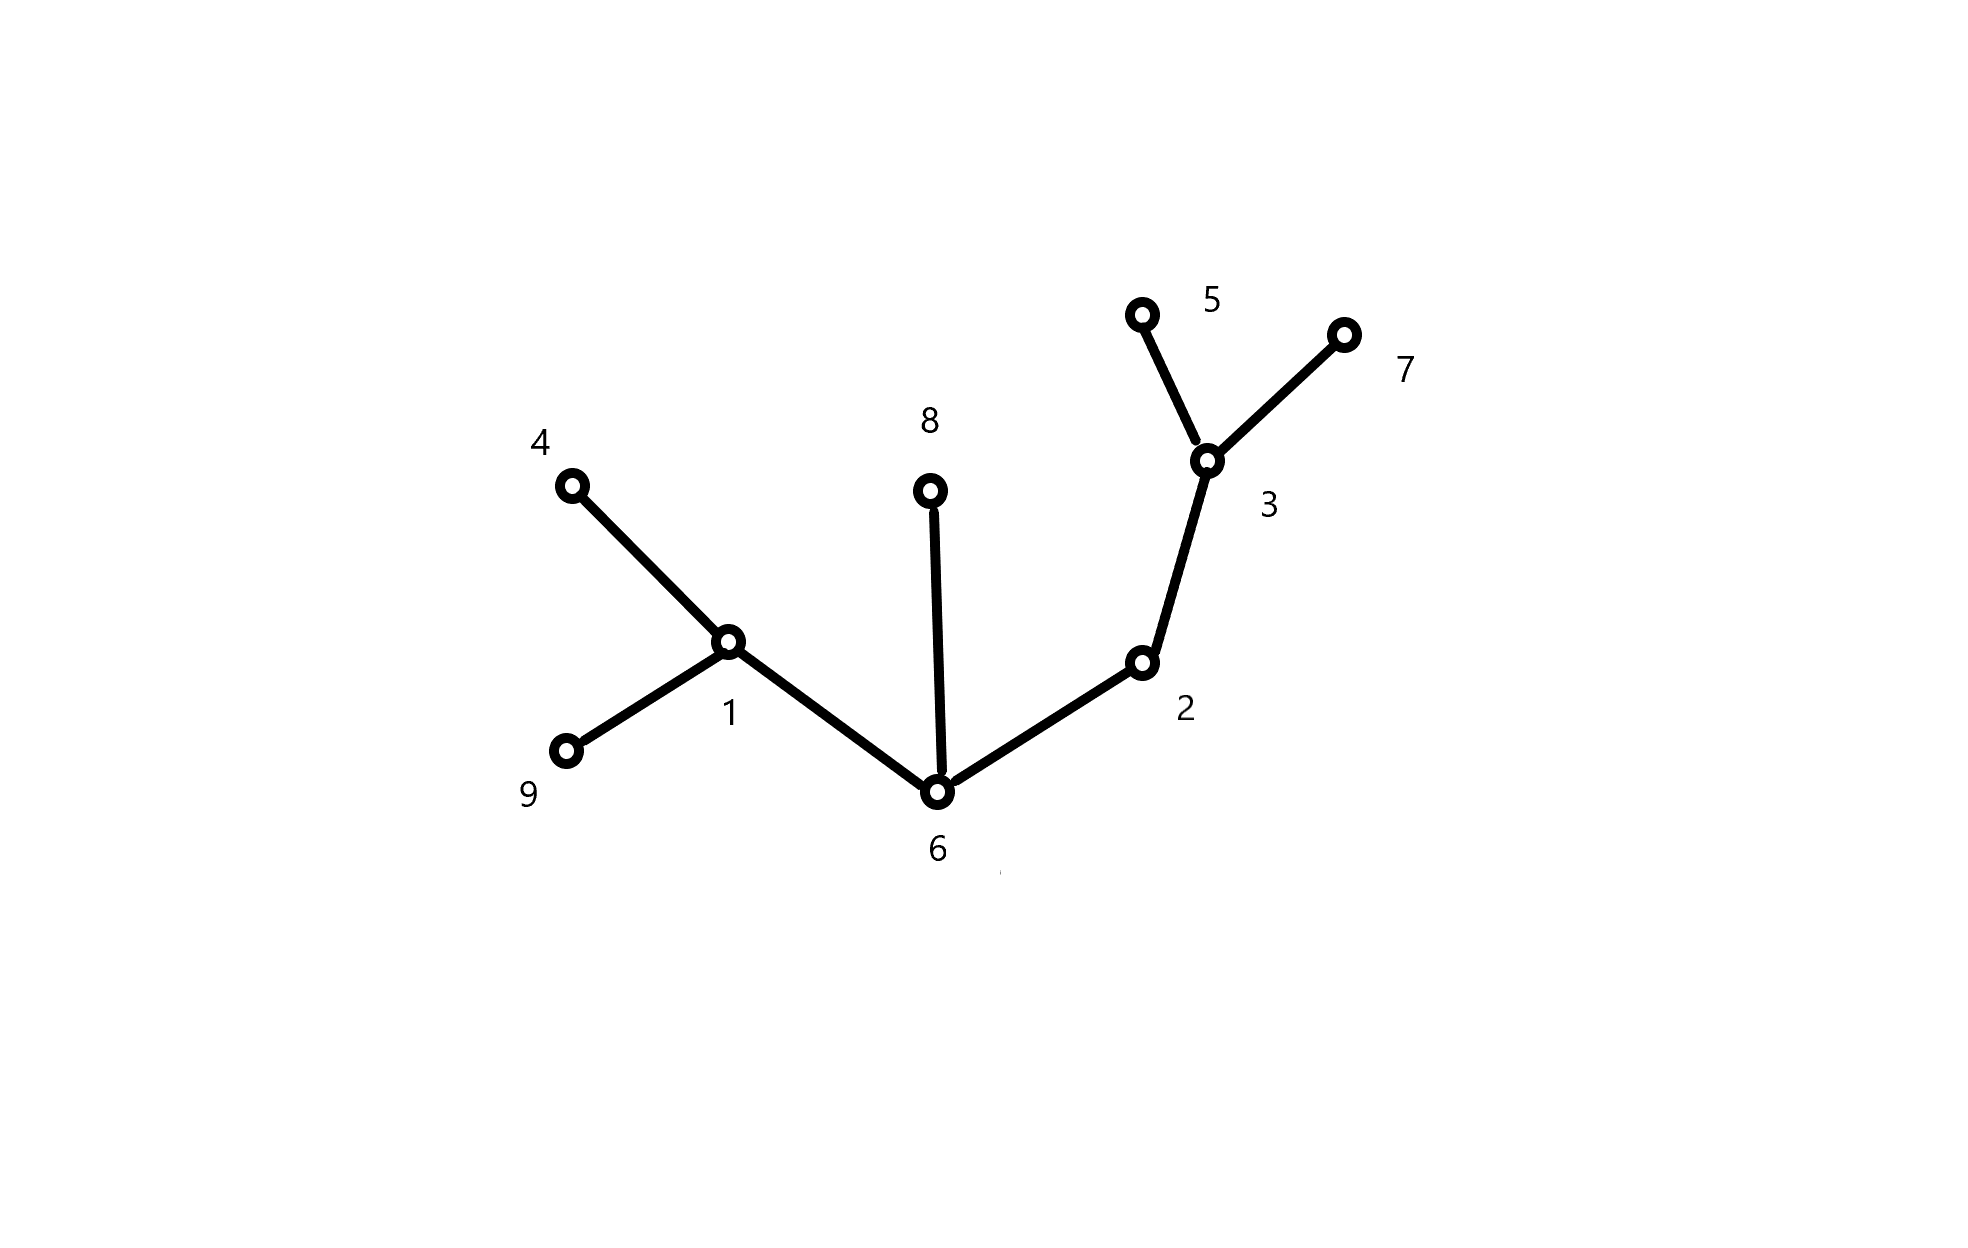
\includegraphics[width=0.9\textwidth]{13_0.png}
  \end{center}
\end{figure}
\end{proof}
\begin{exercise}
  Let $\mathbf{p} = (p_1,p_2,\dots,p_{n-2})$ be the Pr\"ufer  code of some tree $T$ on $[n]$.
  Find a way to quickly determine the degree of vertex $i$ only by looking
  at $\mathbf{p}$ and not actually constructing the tree $T$.
  In particular, by looking at $\mathbf{p}$, what are the leaves of $T$?
\end{exercise}

\begin{proof} \quad
  \begin{enumerate}
    \item
    The degree of vertex $i$ $=$ 1 + the number of times that $i$ appears in $\mathbf{p}$.
    \item
    Vertex $i$ is a leave if and only if $i$ does not appear in $\mathbf{p}$.
  \end{enumerate}

\end{proof}

\begin{exercise}
  Describe which tree on $V = [n]$  has the
  \begin{enumerate}
  \item Pr\"ufer code $(1,1,\dots,1)$.
  \item Pr\"ufer code $(1,2,3,\dots, n-2)$.
  \item Pr\"ufer code $(3,4,5,\dots, n)$.
  \item Pr\"ufer code $(n, n-1, n-2,\dots,4,3)$.
  \item Pr\"ufer code $(n-2,n-3,\dots,2,1)$.
  \item Pr\"ufer code $(1,2,1,2,\dots,1,2)$ (assuming $n$ is even).
 \end{enumerate}
 Justify and explain your answers.
 \begin{proof}
  \begin{enumerate}
    \item
    The constructing process is shown as Table \ref{151}.
    \begin{table}[H]
      \caption{}\label{151}
      \begin{center}
  \begin{tabular*}{6cm}{l|l|l}
  \hline
  V & Code  & Leaf \\
  \hline
  12 $\cdots$ n  & 1 $\cdots$ 1 & 2 \\
  134 $\cdots$ n  & 1 $\cdots$ 1 & 3 \\
  \vdots & \vdots & \vdots \\
  1(n-1)n & 1 & n-1 \\
  1n &  &  \\
  \hline
  \end{tabular*}
  \end{center}
  \end{table}

  The tree is shown as following.
  \begin{figure}[H]
    \begin{center}
    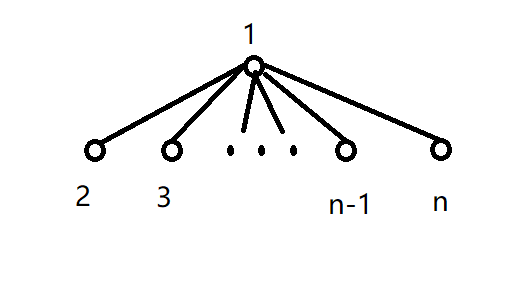
\includegraphics[width=0.5\textwidth]{151.png}
    \end{center}
  \end{figure}

  \item
  The constructing process is shown as Table \ref{152}.
  \begin{table}[H]
    \caption{}\label{152}
    \begin{center}
\begin{tabular*}{8cm}{l|l|l}
\hline
V & Code  & Leaf \\
\hline
12 $\cdots$ n  & 1 $\cdots$ (n-2) & (n-1) \\
12 $\cdots$ (n-2)n  & 2 $\cdots$ (n-2) & 1 \\
23 $\cdots$ (n-2)n  & 3 $\cdots$ (n-2) & 2 \\
\vdots & \vdots & \vdots \\
(n-3)(n-2)n & (n-2) & (n-3) \\
(n-2)n &  &  \\

\hline
\end{tabular*}
\end{center}
\end{table}

The tree is shown as following.
\begin{figure}[H]
  \begin{center}
  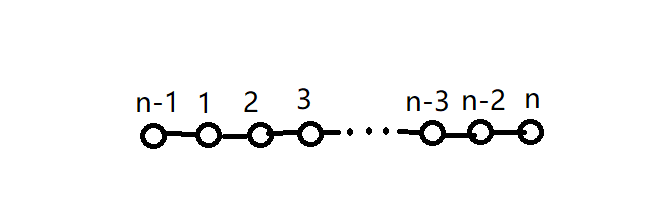
\includegraphics[width=0.5\textwidth]{152.png}
  \end{center}
\end{figure}

\item
The constructing process is shown as Table \ref{153}.
\begin{table}[H]
  \caption{}\label{153}
  \begin{center}
\begin{tabular*}{8cm}{l|l|l}
\hline
V & Code  & Leaf \\
\hline
12 $\cdots$ n  & 34 $\cdots$ n & 1 \\
23 $\cdots$ n  & 45 $\cdots$ n & 2 \\
\vdots & \vdots & \vdots \\
(n-2)(n-1)n & n & (n-2) \\
(n-1)n &  &  \\

\hline
\end{tabular*}
\end{center}
\end{table}

The tree is shown as following.
\begin{figure}[H]
\begin{center}
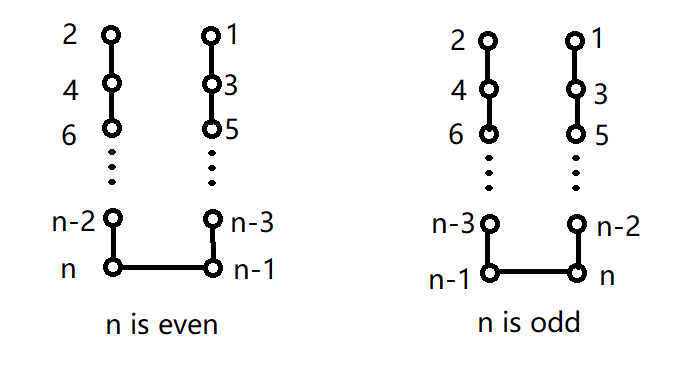
\includegraphics[width=0.5\textwidth]{153.png}
\end{center}
\end{figure}

\item
The constructing process is shown as Table \ref{154}.
\begin{table}[H]
  \caption{}\label{154}
  \begin{center}
\begin{tabular*}{8cm}{l|l|l}
\hline
V & Code  & Leaf \\
\hline
12 $\cdots$ n  & n(n-1) $\cdots$ 3 & 1 \\
23 $\cdots$ n  & (n-1)(n-2) $\cdots$ 3 & 2 \\
34 $\cdots$ n  & (n-2)(n-3) $\cdots$ 3 & (n-1) \\
34 $\cdots$ (n-2)n & (n-3)(n-4) $\cdots$ 3 & (n-2) \\
\vdots & \vdots & \vdots \\
345n & 43 & 5 \\
34n  & 3  & 4 \\
3n & & \\


\hline
\end{tabular*}
\end{center}
\end{table}

The tree is shown as following.
\begin{figure}[H]
\begin{center}
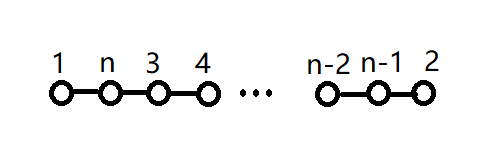
\includegraphics[width=0.5\textwidth]{154.png}
\end{center}
\end{figure}

\item
The constructing process is shown as Table \ref{155}.
\begin{table}[H]
  \caption{}\label{155}
  \begin{center}
\begin{tabular*}{8cm}{l|l|l}
\hline
V & Code  & Leaf \\
\hline
12 $\cdots$ n  & (n-2)(n-3) $\cdots$ 1 & (n-1) \\
12 $\cdots$ (n-2)n  & (n-3)(n-4) $\cdots$ 1 & (n-2) \\
12 $\cdots$ (n-3)n  & (n-4)(n-5) $\cdots$ 1 & (n-3) \\
\vdots & \vdots & \vdots \\
123n & 21 & 3 \\
12n  & 1  & 2 \\
1n & & \\


\hline
\end{tabular*}
\end{center}
\end{table}

The tree is shown as following.
\begin{figure}[H]
\begin{center}
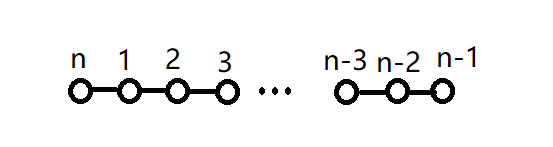
\includegraphics[width=0.5\textwidth]{155.png}
\end{center}
\end{figure}

\item
The constructing process is shown as Table \ref{156}.
\begin{table}[H]
  \caption{}\label{156}
  \begin{center}
\begin{tabular*}{8cm}{l|l|l}
\hline
V & Code  & Leaf \\
\hline
12 $\cdots$ n  & 1212 $\cdots$ 12 & 3 \\
124 $\cdots$ n  & 2121 $\cdots$ 12 & 4 \\
125 $\cdots$ n  & 1212 $\cdots$ 12 & 5 \\
\vdots & \vdots & \vdots \\
12(n-1)n & 12 & (n-1) \\
12n  & 2  & 1 \\
2n & & \\


\hline
\end{tabular*}
\end{center}
\end{table}

The tree is shown as following.
\begin{figure}[H]
\begin{center}
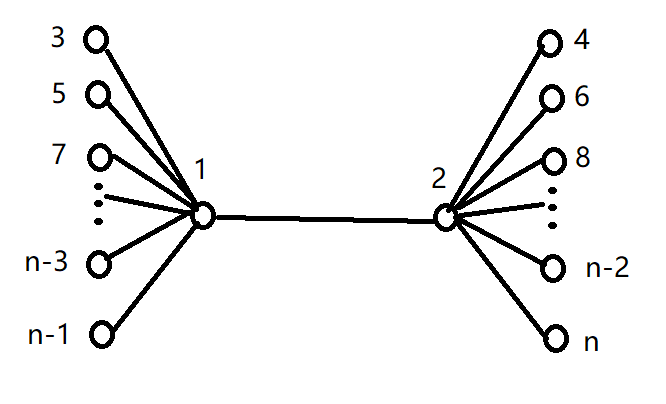
\includegraphics[width=0.5\textwidth]{156.png}
\end{center}
\end{figure}
  \end{enumerate}
\end{proof}
\end{exercise}


  

The next two exercises use a bit of probability theory. Suppose we want to sample a random
tree on $[n]$. That is, we want to write a little procedure (say in Java) that uses randomness and outputs
a tree $T$ on $[n]$, where each of the $n^{n-2}$ trees has the same probability of 
appearing. 

\begin{exercise}
   Sketch how one could write such a procedure. Don't actually write program code, just
   describe it informally. You can assume you have access to a random generator
   \texttt{randomInt($n$)} that returns a function in $\{1,\dots,n\}$ as well
   as \texttt{randomReal()} that returns a random real number from the interval $[0,1]$.

\begin{solution} 
	Randomly create a sequence $(p_1, p_2, \cdots , p_{n-2})$, with $1 \leq p_i \leq n$. We can regard this sequence as prüfer code to construct a tree.
\end{solution}
\end{exercise}



Clearly, a tree $T$ on $[n]$ has at least $2$ and at most $n-1$ leaves. But how 
many leaves does it have on average? For this, we could use your tree sampler from the previous
exercise, run it 1000 times and compute the average. However, it would be much nicer to have 
a closed formula.

\begin{exercise}
  Fix some vertex $u \in [n]$. If we choose a tree $T$ on $[n]$ uniformly at random,
  what is the probability that $u$ is a leaf?
   What is the expected number of leaves of $T$?\
\begin{solution} \quad
\begin{enumerate}
	\item Number the vertices of tree $T$ from 1 to n. We can derive the prüfer code $(p_1, p_2, \cdots , p_{n-2})$ of the tree $T$, with $1 \leq p_i \leq n$. If $u$ is a leaf, then $u$ cannot appear in the prüfer code. 
	$$P[\text{$u$ is a leaf}] = (n - 1) ^ {n - 2} / n ^ {n - 2} = (\frac{n-1}{n})^{n-2}$$
	\item The number of leaves prüfer code of $T$ is denoted by the number of vertices which don't appear in the prüfer code.
  $$
    \mathbb{E}[\text{number of leaves of $T$}] = \sum\limits_{k = 1} ^ {n - 2} \frac{(n - k)(\binom{n}{k}k^{n-2} - \frac{n-k+1}{k-1}\binom{n}{k-1}(k-1)^{n-2})}{n ^ {n - 2}}
  $$
\end{enumerate}
\end{solution}
\end{exercise}

\begin{exercise}
  For a fixed vertex $u$, what is the probability that $u$ has degree $2$?
\begin{solution}
  $$P[\text{$u$ has degree $2$}] = (n - 1) ^ {n - 3} \times 1 \times (n - 2) / n ^ {n-2} = \frac{(n-2)(n - 1) ^ {n - 3}}{n ^ {n-2}}$$
\end{solution}
\end{exercise}







\end{document}
